\section{Downstream Dependency Mining}
\label{sec:approach}

To improve the developers' knowledge about the usages of their packages, our goal is to build a system that allows package developers to survey the API usage of downstream dependencies for a chosen target package.
Concretely, we have identified three common questions of package developers about the usage of their packages:

\begin{enumerate}[label=Q\arabic*]
	\item \label[question]{q1} Which dependencies are using the target package, and what problems do they attempt to solve with it?
	\item \label[question]{q2} By how many dependencies is a particular package member being used?
	\item \label[question]{q3} In which contexts and constellations is a particular package member being used?
\end{enumerate}

Furthermore, we pose two organizational requirements to the eventual tool solution to ensure its practical applicability for the target user group:

\begin{enumerate}[label=R\arabic*]
	\item \label[requirement]{req1} The tool runs out-of-the-box with a small footprint, without the user needing to perform any sophisticated setup steps or providing additional system resources.
	\item \label[requirement]{req2} The tool blends in with the usual workflow of package developers at the best possible rate.
\end{enumerate}

In the following, we will describe both steps of our approach to collect the desired data.

\subsection{Downstream Dependency Collection}
\label{sec:approach/dependency_collection}

In the first step, a list of repositories that depend on the target package has to be assembled.
As mentioned in \cref{sec:related_work/usage_samples}, many approaches start with a large downloaded corpus of unspecific repositories from the ecosystem, which they then iterate over to filter the relevant repositories.
However, a major drawback of this approach is the high resource demand for both creating and traversing this corpus.
This approach is suited for analyzing repositories on a large scale but is not conform to \cref{req1} because of its large footprint in terms of computational power and time.

As an alternative, we have decided to apply significant pre-filtering to the set of repositories before downloading a subset of it to the local machine.
For that, we have identified two types of data sources that are available in public clouds:

\begin{enumerate}[label=(\roman*)]
	\item Package repositories that maintain a doubly-connected edge list of interdependent packages in an ecosystem.
	\item Code search engines that index the source code of many repositories from OSS platforms.
		Using these search engines, we can query all repositories that declare a dependency on the target package in their package manifest file.
\end{enumerate}

\subsection{Usage Sample Mining}
\label{sec:approach/usage_mining}

\begin{figure*}
	\begin{minipage}{\linewidth}
		\colorlet{lowlight}{black!40}
		\newcommand\textlowlight[1]{\textcolor{lowlight}{#1}}
		\newcommand\texthighlight[1]{\textbf{\textcolor{accent1}{#1}}}
		\begin{center}
			\begin{subfigure}[t]{.32\linewidth}
				\begin{tikzpicture}
	\node {CallExpression}
		child {node [accent1] {identifier}}
		child [gray] {node [gray, yshift = -0.5cm] {typeArguments}}
		child [gray] {node [gray] {arguments}};
\end{tikzpicture}
\caption[LoF entry]{
	Node pattern for a TypeScript functional call, such as in:

	\code{\textlowlight{result = }\uline{\texthighlight{fun}<\textlowlight{T1}, \textlowlight{T2}>(\textlowlight{arg1}, \textlowlight{arg2})}\textlowlight{;}}
}

			\end{subfigure}
			\hfill
			\begin{subfigure}[t]{.32\linewidth}
				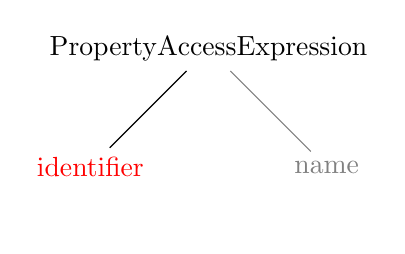
\begin{tikzpicture}
	\node {PropertyAccessExpression}
		child {node [red] {identifier}}
		child [white] {node [yshift = -0.5cm] {\phantom{node}}}  % ensure same height as sibling figures
		child [gray] {node [gray] {name}}
		;
\end{tikzpicture}
\caption[LoF entry]{
	Node pattern for a property access, such as in:

	\code{\lowlight{return }\uline{\lowlight{obj}.\highlight{prop}}\lowlight{;}}
}

			\end{subfigure}
			\hfill
			\begin{subfigure}[t]{.32\linewidth}
				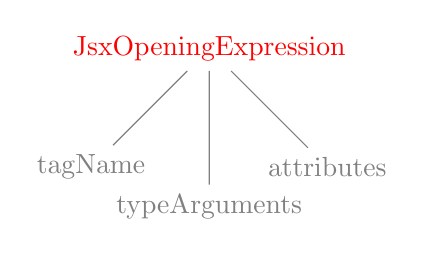
\begin{tikzpicture}
	\node [red] {JsxOpeningExpression}
		child [gray] {node [gray] {tagName}}
		child [gray] {node [gray, yshift = -0.5cm] {typeArguments}}
		child [gray] {node [gray] {attributes}};
\end{tikzpicture}
\caption[LoF entry]{
	Node pattern for a JSX opening element (as supported in React\protect\footnotemark{} or TypeScript\protect\footnotemark{}), such as in:
	\code{\lowlight{elem = }\uline{<Button \lowlight{color}="\lowlight{blue}"> \lowlight{Google</Button>}}\lowlight{;}}
}

			\end{subfigure}

			\caption{AST patterns for example JavaScript/TypeScript expressions.
				The \texthighlight{highlighted} node contains the link to the declaration of the referenced identifier.
			}
			\label{fig:approach/usage_mining/patterns}
		\end{center}
	\end{minipage}
\end{figure*}

Having downloaded the selected downstream dependency repositories, we can proceed to extract usage samples for the target package from each dependency repository.
Our goal is to collect fine-grained source code excerpts that reference single identifiers exposed by the target package.
The complete procedure is displayed in \cref{alg:usage_mining}.

\begin{algorithm}[b]
	\caption{Extraction of usage samples.}\label{alg:usage_mining}

	\KwIn{\\\Indp
		$\mli{pkg}$: target package \\
		$\mli{dependencies}$: downstream dependencies}
	\KwOut{usage samples (set of strings)}
	\;
	\For{$\mli{dep} \in \mli{dependencies}$}{
		$\mli{asf} \gets \mtx{parse}(\mli{dep} \cup \mli{pkg})$\;
	  	$\mtx{annotate\_types}(\mli{asf})$\;
		\For{$\mli{ast} \in \mli{asf}$}{
			\For{$\mli{node} \in \mli{dfs}(\mli{ast})$}{
				\For{$\mli{pattern} \in \mli{patterns}$}{
					\If{$\mli{pattern}.\mtx{matches}(\mli{node}) \wedge \mli{pkg}.\mtx{declares}(\mli{pattern}.\mtx{getType}(\mli{node}))$}{
						\kwYield{$\mli{node}.\mtx{text}$}
					}
				}
			}
		}
	}
\end{algorithm}

To do so, we start by parsing the source code of every dependency repository as well as the source code of the target package each into a separate \emph{abstract syntax forest} (ASF, i.e., a set of ASTs).

In a second step, we perform a static type analysis against each dependency ASF together with the target package's ASF.
The results of the type analysis are attached to the ASF so that every identifier is annotated with a type symbol that links to the declaration of the type for the identifier.
For instance, after this step, every variable node will contain a link to the assignment node of this variable, and every function call expression will contain a link to the definition of this function.
The operating principle of this type analysis depends on the kind of programming language; that is, in statically typed languages, type symbols can usually be retrieved from the declaration of an identifier, whereas in dynamically typed languages, a control flow analysis will be required to identify the origin of every identifier's type.

In the final step, from each ASF, we collect all nodes whose type is declared in the target package.
To identify these links, we define a set of language-specific patterns for AST subtrees that constitute a usage expression.
In particular, each of these patterns expects a node containing a link to an identifier declaration (see \cref{fig:approach/usage_mining/patterns}).
